\documentclass[a4paper,titlepage,oneside]{article}

\usepackage{amsmath}
\usepackage{amsfonts}
\usepackage{amssymb}
\usepackage{amsthm}
\usepackage[utf8]{inputenc}
\usepackage[T1]{fontenc}
\usepackage{enumitem}
\usepackage{ngerman}
\usepackage{mathtools}
\usepackage{tikz}
\usepackage{blindtext}
%\usepackage{geometry}

%Formatting
\author{Tanja Kohler}
\title{Testdokument}
%\geometry{verbose,a4paper,tmargin=25mm,bmargin=25mm,lmargin=25mm,rmargin=25mm}


%Defining
\def\C{\ensuremath{\mathbb{C}} }
\def\N{\ensuremath{\mathbb{N}} }
\def\Q{\ensuremath{\mathbb{Q}} }
\def\Z{\ensuremath{\mathbb{Z}} }
\def\R{\ensuremath{\mathbb{R}} }
\def\im{\ensuremath{\imath} }
\def\e{\ensuremath{\mathit{e}}}
\def\WSP{\text{Widerspruch.}}

\newcommand{\fa}{\ensuremath{\forall}}
\newcommand{\ex}{\ensuremath{\exists}}
\newcommand{\abs}[1]{\ensuremath{\left|\:#1\:\right|}}

\def\sp{\hspace{0,1cm}}

\newcommand{\IA}[1][n=0]{\vspace{0.1pt}\ensuremath{\text{IA}\sp#1:}}
\newcommand{\IV}{\vspace{0.1pt}\ensuremath{\text{IV}\sp}}
\newcommand{\IS}[1][n \mapsto n+1]{\vspace{0.1pt}\ensuremath{\text{IS}\sp#1}}

\newcommand{\suminf}[2][n]{\ensuremath{\sum_{#1= 0}^{\infty}{#2}}}
\newcommand{\Suminf}[2][n]{\ensuremath{\sum_{#1=1}^{\infty}{#2}}}

\renewcommand{\liminf}[2][n]{\ensuremath{\lim\limits_{#1 \rightarrow \infty}{#2}}}
\newcommand{\limInf}[2][n]{\ensuremath{\lim\limits_{#1 \rightarrow -\infty}{#2}}}
\newcommand{\limnull}[2][n]{\ensuremath{\lim\limits_{#1 \rightarrow 0}{#2}}}

\newcommand{\menge}[2]{\ensuremath{\{#1\sp : \sp #2\}}}

\newcommand{\toinf}[1]{#1 \to \infty}
\newcommand{\longtoinf}[1][n]{\ensuremath{\overset{\scriptscriptstyle{#1 \to \infty}}{\longrightarrow}}}

\newtheoremstyle{thmstyle}{}{0.5cm}{}{}{\bfseries}{}{\newline}{\thmnumber{#2. }\thmname{#1}\quad\thmnote{ #3}\vspace{0.1cm}}

\theoremstyle{thmstyle}
\newtheorem{satz}{Satz}[subsection]
\newtheorem{korr}[satz]{Korollar}
\newtheorem{prop}[satz]{Proposition}
\newtheorem{defi}[satz]{Definition}
\newtheorem{bsp}[satz]{Beispiel}
\newtheorem{bem}[satz]{Bemerkung}

\renewcommand{\proofname}{\textbf{Beweis:}}
\renewcommand{\qedsymbol}{\textit{q.e.d.}}

%Documentstart
\begin{document}

Abstand zwischen Formel und Text

\[ j \left ( m + \sum a\cdot \smash{\underbrace{(b+c)}_{Term 1}}\right)%
  \vphantom{\underbrace{(b+c)}_{Term 1}}% damit Abstand danach stimmt
\]
\blindtext

\[ j \left ( m + \sum a\cdot \smash{\underbrace{(b+c)}_{Term 1}}\right) \]
\blindtext


\[
0+\lefteqn{\overbrace{\phantom{1+2+3}}}1+
\underbrace{2+3+\overbrace{x+y+z}+
\lefteqn{\overbrace{\phantom{4+5}}}4}+5
\]

\(^{3}_{2}\mathsf{O}_{1}^{4}\)

\begin{enumerate}
\item \(\to\)
\item $(a_n)$
\item \( \liminf{a_n} \)
\item $\displaystyle{\Suminf[k]{\frac{1}{k(k+1)}} = 1} $
\item \longtoinf[k]
\end{enumerate}
\[\liminf{a_n}\]
\[\suminf{a_n}\]

MMMMMMMMMMMMMMMMMM \\
MMMMMM		$\displaystyle \liminf{n} a + b$	 	MMMMMM\\
MMMMMMMMMMMMMMMMMM\\
MMMMMM		$\textstyle \liminf{n} a + b$ 		MMMMMM\\
MMMMMMMMMMMMMMMMMM\\
MMMMMM		$\scriptstyle \liminf{n} a + b $ 		MMMMMM\\
MMMMMMMMMMMMMMMMMM\\
MMMMMM 	$\scriptscriptstyle \liminf{n} a + b$ 	MMMMMM\\
MMMMMMMMMMMMMMMMMM\\

\IA \\
\IV \\
\IS \\

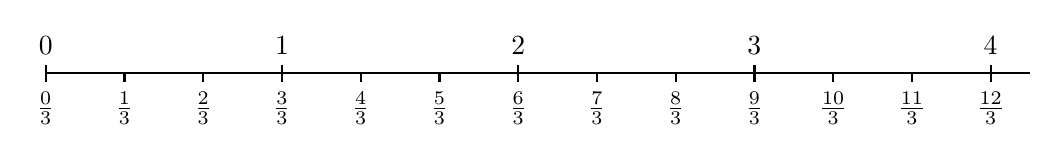
\begin{tikzpicture}[thick]
\newline
    \draw(0,0)--(12.5,0);
    \foreach \x/\xtext in {0/0,3/1,6/2,9/3,12/4}
      \draw(\x,0pt)--(\x,3pt) node[above] {\xtext};
    \foreach \x in {0,1,...,12}
      \draw(\x,0pt)--(\x,-3pt) node[below] {$\frac{\x}{3}$};
  \end{tikzpicture}

\begin{center}
\begin{tikzpicture}
        \draw[step=1,help lines,black!0] (-1,-1) grid (4,4);
        \draw[->] (-0.5,0) -- (3.5,0)  node[below right] {$Re(z)$};
        \draw[->] (0,-0.5) -- (0,3.5)  node[above left]{$Im(z)$};
        \foreach \Point/\PointLabel in {(0,1)/{\im}, (1,0)/1, (2.21,1.75)/{z=(a,b)}}
        \draw[fill=black] \Point circle (0.05) node[above right] {$\PointLabel$};
        \foreach \Point/\PointLabel in {(2.21,0)/a, (0,1.75)/b}
        \draw \Point circle (0.05) node[above right] {$\PointLabel$};
\end{tikzpicture}
\end{center}


\end{document}
